\documentclass[xcolor=dvipsnames]{beamer}
\usepackage{xltxtra}
\usepackage[english]{babel}
\usepackage{listings}

\xdefinecolor{thecolor}{rgb}{0.5,0.0,0.5}

\mode<presentation>
{
	\usetheme{Rochester}
	\beamertemplatenavigationsymbolsempty
	\usecolortheme[named=thecolor]{structure}
	\setbeamercovered{transparent}
}

\title{SDCC}
\subtitle{ISO C Standard Compliance}
\date{2025-04-11}

\author{Benedikt Freisen}

\subject{Small Device C Compiler, SDCC, C, ISO C}

\begin{document}

\begin{frame}
	\titlepage
\end{frame}

\begin{frame}
	\frametitle{Structure of this talk}
	This talk will outline the status quo and objectives surrounding C standard compliance in SDCC, structured as follows:
	\begin{itemize}
		\item Motivation: Why ISO C?
		\item Recent Achievements
		\item Work(s) in Progress
        \item Challenges
        \item Modern C --- Examples
        \item Future Construction Sites
        \item Time for Questions / Feedback / Live Demo
	\end{itemize}
	
\end{frame}

\begin{frame}
	\frametitle{Motivation: Why ISO C?}
	The C programming language was originally standardized by ANSI in 1989, all subsequent versions by ISO
	\begin{itemize}
		\item Features: Language extensions for new use cases
		\item Compatibility: Prevention of diverging dialects
	\end{itemize}
	Therefore, we want a Standard C compiler! (ISO C90 - C2Y)

	Obvious challenge: Standard C is constantly evolving
\end{frame}

\begin{frame}
	\frametitle{Recent Achievements (pre 4.5.0)}
	Six out of the seven new features in 4.5.0 were related to current and future standard compliance:
	\begin{itemize}
		\item Full atomic\_flag support for msc51 and ds390 ports
		\item (Experimental f8 port)
		\item ISO C2y case range expressions
		\item ISO C2y \_Generic selection expression with a type operand
		\item K\&R-style function syntax (preliminarily with the semantics of non-K\&R ISO-style functions)
		\item ISO C23 enums with user-specified underlying type
		\item struct / union in initializers
	\end{itemize}
\end{frame}

\begin{frame}
	\frametitle{Recent Achievements (post 4.5.0)}
	Five out of the six features added since 4.5.0 relate to ISO C, one to GNU C:
	\begin{itemize}
		\item C2y \_Countof operator
		\item C2y octal
		\item C2y if-declaration
		\item Conditional operator with omitted second operand (GNU extension)
		\item C99 compound literals
		\item C23 compound literals with storage class specifiers
	\end{itemize}
\end{frame}

\begin{frame}
	\frametitle{Work(s) in Progress}
	Various ISO C features have already been worked on, but are not yet complete, e.g.:
	\begin{itemize}
		\item C23 constexpr, i.e. named compile-time constant expressions
		\item C23 qualifier-preserving library functions
		\item C90 flat initializer lists for nested arrays
		\item C23 checked integer arithmetic for 64 bit types
	\end{itemize}
\end{frame}

\begin{frame}
	\frametitle{Challenges}
	There are obstacles preventing the speedy implementation of the aforementioned features:
	\begin{itemize}
		\item Qualifier-preserving wrapper macros rely on \_Generic and ?: specifics that are inaccurately implemented
		\item Flat initilizer lists can contain (top level) element designators, but we have a bottom-up parser
		\item constexpr must not trip over identifier shadowing
		\item 64 bit checked integer arithmetic must make do with 64 bit intermediate values
	\end{itemize}
\end{frame}

\begin{frame}[fragile]
	\frametitle{Challenges: Flat Array Initializer Lists}
	ANSI/ISO C inherits the K\&R C bug/feature that initializer lists may ignore an array type's structure. This is valid:
\begin{lstlisting}[language=C,basicstyle=\footnotesize]
int array[2][2] = { 1, 2, 3 };
\end{lstlisting}
However, ISO C99 added the ability to designate specific array members:
\begin{lstlisting}[language=C,basicstyle=\footnotesize]
int array[2][2] = { 1, [2] = 2, 3 };
\end{lstlisting}
Mixing both means trouble! (At least for compiler devs)
\end{frame}

\begin{frame}[fragile]
	\frametitle{Modern C --- Examples: \_Generic}
	Generics (since C11) allow selecting expressions based on the type of a controlling expression:
\begin{lstlisting}[language=C,basicstyle=\footnotesize]
_Generic(i, default : 0, int : 1, long : 2)
\end{lstlisting}
C2y will add the ability to select based on a type itself, which, combined with C23's \texttt{typeof} permits selection based on the \textit{qualified} type:
\begin{lstlisting}[language=C,basicstyle=\footnotesize]
_Generic(typeof(i), int : 0, const int : 1, default : 2)
\end{lstlisting}

\end{frame}

\begin{frame}[fragile]
	\frametitle{Modern C --- Examples: \texttt{typeof} with function pointers}
	C23's \texttt{typeof} permits a more intuitive spelling of function pointers:
\begin{lstlisting}[language=C,basicstyle=\footnotesize]
void (*signal(int sig, void (*func)(int)))(int);
\end{lstlisting}
becomes
\begin{lstlisting}[language=C,basicstyle=\footnotesize]
typeof(void (int)) *signal(int sig, typeof(void (int)) *func);
\end{lstlisting}
But SDCC does not like this syntax, yet. :-/
\end{frame}

\begin{frame}[fragile]
	\frametitle{Modern C --- Examples: \texttt{case} ranges}
	C2y will \textit{finally} standardize GNU C's \texttt{case} ranges:
\begin{lstlisting}[language=C,basicstyle=\footnotesize]
switch (a) {
    case 0 ... 5: foo(); break;
    case 6 ... 10: bar(); break;
    default: baz(); break;
}
\end{lstlisting}
The implementation in SDCC is based on a user-contributed patch. Those are welcome!\footnote{Particularly when a feature has been standardized}
\end{frame}

\begin{frame}
	\frametitle{Modern C --- Examples: Octal Literals}
	Octal literals in C are notoriously unintuitive, as demonstrated by this pencil "correction" in a library copy of the book "The C Programming Language":
	\centerline{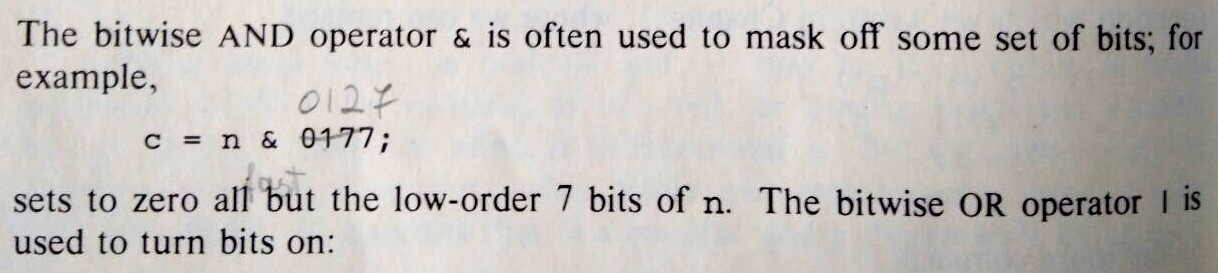
\includegraphics[scale=0.8]{octal.jpg}}
	C2y will allow the more obviously prefixed spelling \texttt{0o177} known from languages like Rust.

	It will also allow escape sequences like "\textbackslash o\{177\}".
\end{frame}

\begin{frame}
	\frametitle{Future Construction Sites}
	Besides the points that are already being worked on, the following ones remain:
	\begin{itemize}
		\item Changes to lexer and parser for better C23 attribute support
		\item Proper IEEE 754 floating point types and library
		\item Whatever the committee decides to put in C2y, e.g.
		\begin{itemize}
			\item Lambda expressions (subset of what C++ has)
			\item Deferred blocks (executed at the end of the containing block)
			\item Named loops (allowing e.g. \texttt{\textbf{continue} outer;})
		\end{itemize}
	\end{itemize}
	All of the above will presumably come with their own unique challenges.
\end{frame}

\begin{frame}
	\frametitle{Time for Questions / Feedback / Live Demo}
	
	\begin{itemize}
		\item Any questions?
		\item Do you have feedback or suggestions?
		\item Would you like to see details?
	\end{itemize}
\end{frame}

\end{document}

